\section{Sch1Eval Class Reference}
\label{classSch1Eval}\index{Sch1Eval@{Sch1Eval}}
Inheritance diagram for Sch1Eval::\begin{figure}[H]
\begin{center}
\leavevmode
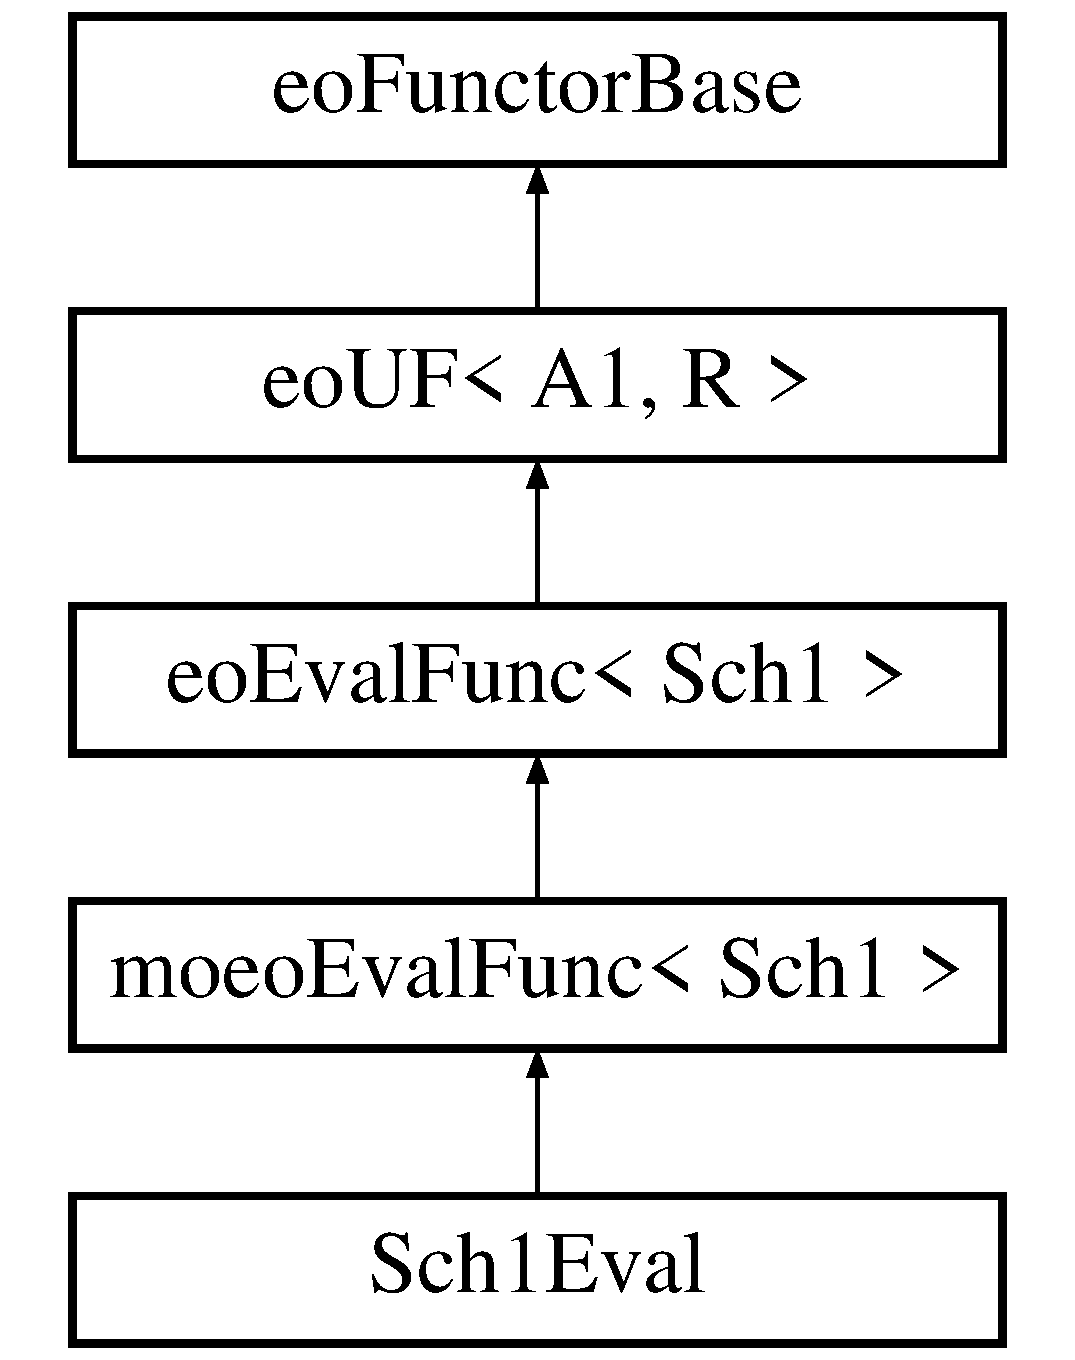
\includegraphics[height=5cm]{classSch1Eval}
\end{center}
\end{figure}
\subsection*{Public Member Functions}
\begin{CompactItemize}
\item 
void \bf{operator()} (\bf{Sch1} \&\_\-sch1)\label{classSch1Eval_4f806a964f7bafa9e4fcca45da458c98}

\end{CompactItemize}


\subsection{Detailed Description}




Definition at line 78 of file Sch1.cpp.

The documentation for this class was generated from the following file:\begin{CompactItemize}
\item 
Sch1.cpp\end{CompactItemize}
